\PassOptionsToPackage{bookmarks={true}}{hyperref}
\pdfminorversion=4
\documentclass[mathserif,xcolor={dvipsnames,table}]{beamer}
\mode<presentation>{\usetheme{Warsaw}\usecolortheme{crane}}
\usepackage{centernot}
\usepackage{mathabx}
\usepackage{graphicx}
\usepackage{transparent}
\usepackage{geometry}
\usepackage{tikz}
\usetikzlibrary{shadows}
\usepackage[utf8]{inputenc}
\usepackage[english]{babel}
\usepackage[T1]{fontenc}
\usepackage{lmodern}
\usepackage[babel=true]{microtype}
\usepackage{amsmath}
\beamertemplatenavigationsymbolsempty

\title{\textbf{Kernelspace}}
\date{}
\author{CS4803UWS at the\\
Georgia Institute of Technology
}

\begin{document}

{
\setbeamertemplate{background canvas}{%

\includegraphics[width=\paperwidth,height=\paperheight]{images/gt2.jpeg}
}%
\begin{frame}[plain]
\textcolor{white}{
\transparent{0.5}%
\colorbox{black}{\textbf{kernelspace}}
}
\vspace{2.7in}
\\
\hfill
\includegraphics[scale=.25]{images/cc-logo.pdf}

\includegraphics[scale=.25]{images/cc-new.pdf}

\includegraphics[scale=.25]{images/cc-share.pdf}
\textcolor{white}{
\\
\hfill \tiny{CC3.0 share-alike attribution}\\
}
\textcolor{white}{
\hfill \scriptsize{copyright \copyright\ 2013}\\
}
\end{frame}
}

\begin{frame}{Processes}
Process 1\footnote{\tiny{Typically {\tt /sbin/init}; override this with kernel parameter {\tt init=}, i.e. ``{\tt init=/bin/sh}''.}} is launched by the
kernel following initialization. The kernel will panic if {\tt init} cannot be found,
or if process 1 ever terminates. Process 1 is the ultimate ancestor of all userspace
processes, and orphaned processes are reparented to it.
\vfill
On Linux, new processes are launched with {\tt clone(2)}. GNU libc since 2.3.3
implements {\tt fork(2)} in terms of {\tt clone(2)}. FreeBSD uses the more
traditional {\tt rfork(2)} interface. As of FreeBSD 9.1, {\tt fork(2)} is not
implemented in terms of {\tt rfork(2)} ``for reasons of backwards
compatibility.\footnote{\tiny{? Dubious!}}''
\vfill
{\tt vfork(2)} is unnecessary with modern COW implementations, and has been
deprecated by POSIX.1-2008. Do not use it in new code.
\end{frame}

\begin{frame}{POSIX.1-2001 Credentials}
\scriptsize{A process's PID and PPID, real UID, real GID, and supplementary group IDs are
preserved across an {\tt execve(2)}. Effective and set UIDs/GIDs might be
changed. Process groups cannot cross session boundaries.}
\vfill
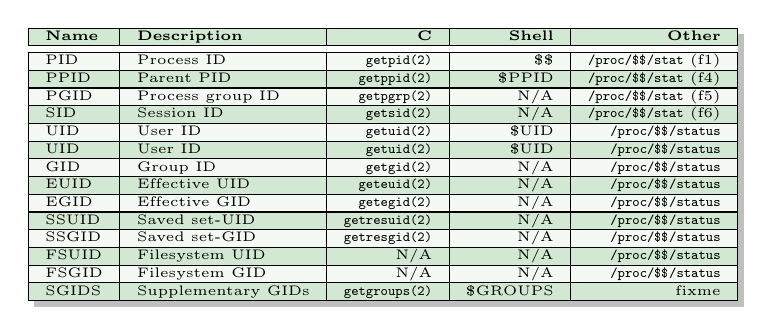
\begin{tikzpicture}
\node[drop shadow,fill=white,inner sep=0pt]
{\rowcolors{1}{ForestGreen!20}{ForestGreen!5}
{\tiny
\begin{tabular}{|l|l|r|r|r|}
\hline
\textbf{Name} & \textbf{Description} & \textbf{C} & \textbf{Shell} & \textbf{Other} \\
\hline\hline
PID & Process ID & {\tt getpid(2)} & \$\$ & {\tt /proc/\$\$/stat} (f1)\\
\hline
PPID & Parent PID & {\tt getppid(2)} & \$PPID & {\tt /proc/\$\$/stat} (f4)\\
\hline
PGID & Process group ID & {\tt getpgrp(2)} & N/A & {\tt /proc/\$\$/stat} (f5)\\
\hline
SID & Session ID & {\tt getsid(2)} & N/A & {\tt /proc/\$\$/stat} (f6)\\
\hline
UID & User ID & {\tt getuid(2)} & \$UID & {\tt /proc/\$\$/status}\\
\hline
UID & User ID & {\tt getuid(2)} & \$UID & {\tt /proc/\$\$/status}\\
\hline
GID & Group ID & {\tt getgid(2)} & N/A & {\tt /proc/\$\$/status}\\
\hline
EUID & Effective UID & {\tt geteuid(2)} & N/A & {\tt /proc/\$\$/status}\\
\hline
EGID & Effective GID & {\tt getegid(2)} & N/A & {\tt /proc/\$\$/status}\\
\hline
SSUID & Saved set-UID & {\tt getresuid(2)} & N/A & {\tt /proc/\$\$/status}\\
\hline
SSGID & Saved set-GID & {\tt getresgid(2)} & N/A & {\tt /proc/\$\$/status}\\
\hline
FSUID & Filesystem UID & N/A & N/A & {\tt /proc/\$\$/status}\\
\hline
FSGID & Filesystem GID & N/A & N/A & {\tt /proc/\$\$/status}\\
\hline
SGIDS & Supplementary GIDs & {\tt getgroups(2)} & \$GROUPS & fixme \\
\hline
\end{tabular}%
}
};
\end{tikzpicture}
\vfill
\scriptsize{Filesystem UID/GID are Linux-specific. Upon an EUID/EGID change,
the kernel changes the FSUID/FSGID to match the new values.}
\vfill
\scriptsize{OS X supports per-thread credentials using {\tt
pthread\_setugid\_np(2)} and {\tt pthread\_getugid\_np(2)}. A {\tt
pthread\_getcred\_np} and {\tt pthread\_setcred\_np} were introduced on the
freebsd-arch mailing list in 2009, but have seen little discussion. Linux
uses per-thread credentials in kernelspace, but NPTL enforces the 1-2001
model.}
\end{frame}

\begin{frame}{POSIX.1e Capabilities}
\footnotesize{The superuser concept is very coarse security. Linux
implements\footnote{\tiny{When the {\tt CONFIG\_SECURITY\_CAPABILITIES} option is used during kernel build.}}
fine-grained per-thread \textit{capabilities} from the withdrawn POSIX.1e standard, and a
wealth of optional ``security models'' (see {\tt CONFIG\_SECURITY}). FreeBSD 9
introduced \textit{capsicum(4)}, a radically different system.}
\begin{center}\footnotesize{\textbf{Linux capabilities as of 3.9}}\end{center}
\tiny{
\begin{columns}
\begin{column}{.33\textwidth}
{\tt
\begin{itemize}
\item CAP\_AUDIT\_CONTROL
\item CAP\_AUDIT\_WRITE
\item CAP\_BLOCK\_SUSPEND
\item \textbf{CAP\_CHOWN}
\item \textbf{CAP\_DAC\_OVERRIDE}
\item CAP\_DAC\_READ\_SEARCH
\item \textbf{CAP\_FOWNER}
\item \textbf{CAP\_FSETID}
\item CAP\_IPC\_LOCK
\item CAP\_IPC\_OWNER
\item \textbf{CAP\_KILL}
\item CAP\_LEASE
\end{itemize}
}
\hfill \textbf{Boldface denotes POSIX.1e.}
\end{column}
\begin{column}{.33\textwidth}
{\tt
\begin{itemize}
\item CAP\_LINUX\_IMMUTABLE
\item CAP\_MAC\_ADMIN
\item CAP\_MAC\_OVERRIDE
\item CAP\_MKNOD
\item CAP\_NET\_ADMIN
\item CAP\_NET\_BIND\_SERVICE
\item CAP\_NET\_BROADCAST
\item CAP\_NET\_RAW
\item \textbf{CAP\_SETGID}
\item CAP\_SETFCAP
\item CAP\_SETPCAP
\item \textbf{CAP\_SETUID}
\end{itemize}
}
All others are Linux-specific.
\end{column}
\begin{column}{.33\textwidth}
{\tt
\begin{itemize}
\item CAP\_SYS\_ADMIN
\item CAP\_SYS\_BOOT
\item CAP\_SYS\_CHROOT
\item CAP\_SYS\_MODULE
\item CAP\_SYS\_NICE
\item CAP\_SYS\_PACCT
\item CAP\_SYS\_PTRACE
\item CAP\_SYS\_RAWIO
\item CAP\_SYS\_RESOURCE
\item CAP\_SYS\_TIME
\item CAP\_SYS\_TTY\_CONFIG
\item CAP\_SYSLOG
\item CAP\_WAKE\_ALARM
\end{itemize}
}
\end{column}
\end{columns}
}
\end{frame}

\begin{frame}{Namespaces}
Various identifiers are globally shared; each set forms a namespace. Child
processes live in their parents' namespaces by default. On Linux, this 
behavior can be changed via arguments to the {\tt clone(2)} system call at
child creation time. A process can change its own namespaces via
{\tt setns(2)}\footnote{\tiny{Added in kernel 3.0. {\tt setns(2)}
cannot (as of 3.9.2) change all namespaces, only IPC/UTS/Net.}}
\vfill
\hfill
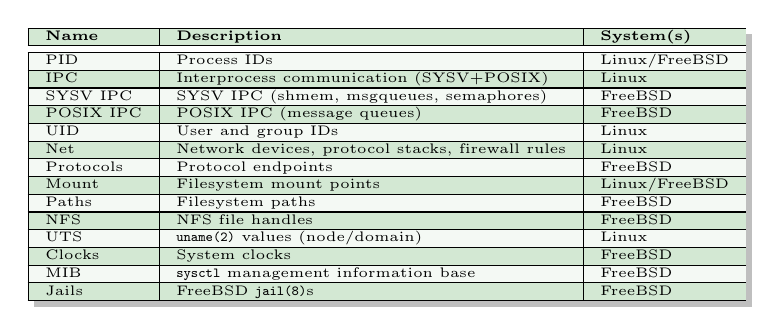
\begin{tikzpicture}
\node[drop shadow,fill=white,inner sep=0pt]
{\rowcolors{1}{ForestGreen!20}{ForestGreen!5}
{\tiny
\begin{tabular}{|l|l|l}
\hline
\textbf{Name} & \textbf{Description} & \textbf{System(s)} \\
\hline\hline
PID & Process IDs & Linux/FreeBSD\\
\hline
IPC & Interprocess communication (SYSV+POSIX) & Linux\\
\hline
$\drsh$SYSV IPC & SYSV IPC (shmem, msgqueues, semaphores) & FreeBSD\\
\hline
$\drsh$POSIX IPC & POSIX IPC (message queues) & FreeBSD\\
\hline
UID & User and group IDs & Linux\\
\hline
Net & Network devices, protocol stacks, firewall rules & Linux\\
\hline
$\drsh$Protocols & Protocol endpoints & FreeBSD\\
\hline
Mount & Filesystem mount points & Linux/FreeBSD\\
\hline
Paths & Filesystem paths & FreeBSD\\
\hline
NFS & NFS file handles & FreeBSD\\
\hline
UTS & {\tt uname(2)} values (node/domain) & Linux\\
\hline
Clocks & System clocks & FreeBSD\\
\hline
MIB & {\tt sysctl} management information base  & FreeBSD\\
\hline
Jails & FreeBSD {\tt jail(8)}s  & FreeBSD\\
\hline
\end{tabular}%
}
};
\end{tikzpicture}
\end{frame}

\end{document}
